\section{The Programmable Storage Challenge}
\label{sec:progly}

When application requirements are not met by an underlying storage system the
most common approach is to design a workaround that will fall roughly into one
of three categories:

{\bf Extra services.} `Bolt-on'' services are intended to improve performance
or enable a feature, but come at the expensive of additional sub-systems and
dependencies that the application must manage, as well as trust.

{\bf Application changes.} The second approach to adapting to a storage system
deficiency is to change the application itself by adding more data management
intelligence into the application or as domain-specific middleware. When
application changes depend on non-standard semantics exposed by the storage
system the coupling that results can be fragile and result in lock-in.

{\bf Storage modifications.} When these two approaches fail to meet an
application's needs, developers may turn their attention to any number of
heavy-weight solutions ranging from changing the storage system itself, up to
and including designing entirely new systems. This approach requires
significant domain knowledge, and extreme care when altering code-hardened
systems.

Rather than relying on storage systems to evolve \emph{or} applications to
change, a hybrid approach that embraces interface instability allows maximum
flexibility, so long as it does not impose an unmanagable burden on
developers.

\subsection{Programmable Storage}

Malacology is a recently proposed approach that advocates a design strategy
called programmable storage in which existing storage system services are
safely exposed such that they can be composed to form application specific
services. Figure~\ref{fig:malacology} shows the architecture of Malacology as
implemented in Ceph, which exposes a variety of low-level internal services
such object interfaces, and cluster metadata management that are in-turn
composed to form a set of new system services that support the requirements of
multiple real-world applications.

\begin{figure}[th]
\centering
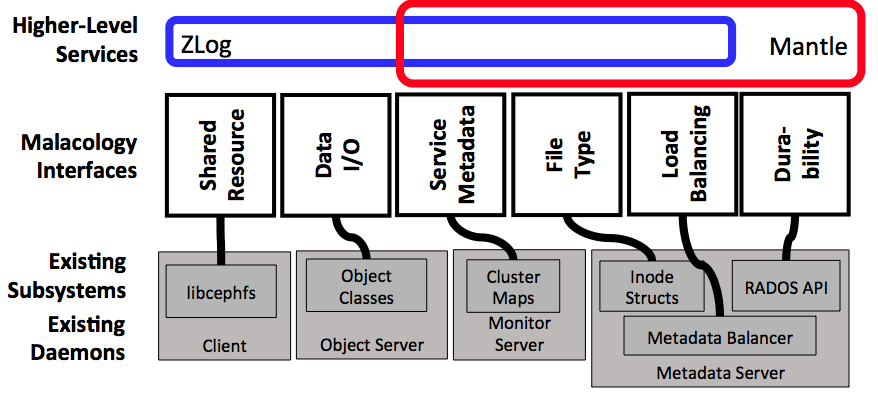
\includegraphics[width=1.0\linewidth]{implementation-overview.png}
\caption{Malacology implementation in Ceph. Existing sub-systems are composed
    to form new services and application-specific optimizations.}
\label{fig:malacology}
\end{figure}

The Malacology services exposed in Ceph were demonstrated by implementing the
CORFU high-performance shared-log abstraction. The design re-used metadata
management caching features to construct the high-frequncy network-attached
counter, and software-defined object interfaces replicated the write-once
semantics of the storage devices, both of which are required by the CORFU
protocol. While the ability to build software-defined interfaces is powerful,
next we will show how access to low-level interfaces can be a double-edged
sword, providing power at the cost of maintenance.

\subsection{Everyone Loves A Standard}

The narrow interface exposed by storage systems has been a boon in allow
systems and applications to evolve independently, in affect limiting the size
of the design space where applications couple with storage. Programmable
storage lifts the veil the system, and with it, forces applications developers
to confront a large set of possible designs.

To illustrate this challenge we implemented as an object interface the CORFU
storage device specification, that is a write-once interface over a 64-bit
address space. The interface is used as a building block of the CORFU protocol
to read and write log entries that are striped over an entire cluster. 
The implementations differ in their optimization strategy of utilizing
internal system interfaces. For instance one implementation uses a key-value
interface to manage the address space index and entry data, while another
implementation stores the entry data using a byte-addressable interface.

\begin{figure}[t]
\centering
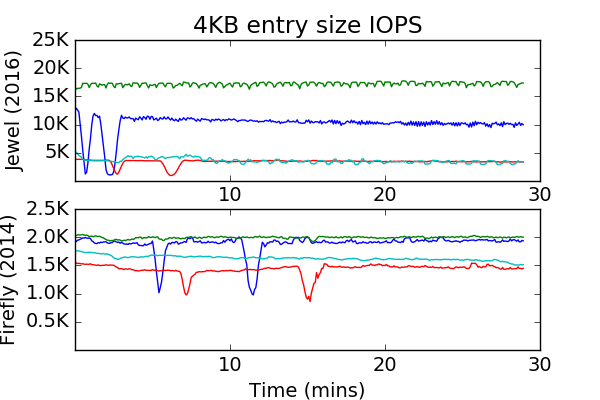
\includegraphics[width=1.0\linewidth]{jewel_v_firefly_pd.png}
\caption{asdf}
\label{fig:phy-design}
\end{figure}

Figure~\ref{fig:phy-design} shows the append throughput of four such
implementations run on two versions of Ceph from 2014 and 2016. The first
observation to be made is that performance in general is significantly better
in the newer version of Ceph. However, what is interesting is the relationship
between the implementations. Run on a version of Ceph from 2014, the top two
implementations perform with nearly identical throughput, but have strikingly
different implementation complexities. The performance of the same
implementations on a newer version of Ceph illustrate a challenge: given a
reasonable choice of a simpler implementation in 2014, a storage interface
will perform worse in 2016, requiring significant rework of low-level
interface implementations.
